\documentclass[letterpaper,12pt]{article}
\usepackage{array}
\usepackage{threeparttable}
\usepackage{geometry}
\geometry{letterpaper,tmargin=1in,bmargin=1in,lmargin=1.25in,rmargin=1.25in}
\usepackage{fancyhdr,lastpage}
\pagestyle{fancy}
\lhead{}
\chead{}
\rhead{}
\lfoot{}
\cfoot{}
\rfoot{\footnotesize\textsl{Page \thepage\ of \pageref{LastPage}}}
\renewcommand\headrulewidth{0pt}
\renewcommand\footrulewidth{0pt}
\usepackage[format=hang,font=normalsize,labelfont=bf]{caption}
\usepackage{listings}
\lstset{frame=single,
  language=Python,
  showstringspaces=false,
  columns=flexible,
  basicstyle={\small\ttfamily},
  numbers=none,
  breaklines=true,
  breakatwhitespace=true
  tabsize=3
}
\usepackage{amsmath}
\usepackage{amssymb}
\usepackage{amsthm}
% \usepackage{harvard}
\usepackage{setspace}
\usepackage{float,color}
\usepackage[pdftex]{graphicx}
\usepackage{hyperref}
\hypersetup{colorlinks,linkcolor=red,urlcolor=blue}
\theoremstyle{definition}
\newtheorem{theorem}{Theorem}
\newtheorem{acknowledgement}[theorem]{Acknowledgement}
\newtheorem{algorithm}[theorem]{Algorithm}
\newtheorem{axiom}[theorem]{Axiom}
\newtheorem{case}[theorem]{Case}
\newtheorem{claim}[theorem]{Claim}
\newtheorem{conclusion}[theorem]{Conclusion}
\newtheorem{condition}[theorem]{Condition}
\newtheorem{conjecture}[theorem]{Conjecture}
\newtheorem{corollary}[theorem]{Corollary}
\newtheorem{criterion}[theorem]{Criterion}
\newtheorem{definition}[theorem]{Definition}
\newtheorem{derivation}{Derivation} % Number derivations on their own
\newtheorem{example}[theorem]{Example}
\newtheorem{exercise}[theorem]{Exercise}
\newtheorem{lemma}[theorem]{Lemma}
\newtheorem{notation}[theorem]{Notation}
\newtheorem{problem}[theorem]{Problem}
\newtheorem{proposition}{Proposition} % Number propositions on their own
\newtheorem{remark}[theorem]{Remark}
\newtheorem{solution}[theorem]{Solution}
\newtheorem{summary}[theorem]{Summary}
%\numberwithin{equation}{section}
\bibliographystyle{aer}
\newcommand\ve{\varepsilon}
\newcommand\boldline{\arrayrulewidth{1pt}\hline}


\begin{document}

\begin{flushleft}
  \textbf{\large{Problem Set \#1}} \\
  MACS 30100, Dr. Evans \\
  Julian McClellan
\end{flushleft}

\vspace{5mm}

\noindent\textbf{Problem 1} 
\newline
\noindent\textbf{Part (a-b).} 
Juhn, Chinhui and Kristin McCue. 2016. "Evolution of the Marriage Earnings Gap for Women." American Economic Review, 106(5): 252-56.

\noindent\textbf{Part (c).} 
$ln Y_{it}=\beta X_{it}+\gamma M_{it}+\pi K_{it}+\delta _{c}+\varepsilon _{it}$
$\varepsilon _{it} = \alpha _{i}+v_{it}$

$i$ indexes the individual, $X$ are observable characteristics such as age, education, race, ethnicity, $M$ is the married dummy, $K$ are indicators for the presence and age of children, $\delta _{c}$ refers to birth cohort effects, and $ln Y_{it}$ refers to the natural log of earnings.

\noindent\textbf{Part (d).}
The only endogenous variable in the model is $ln Y_{it}$, the natural log of the earnings. Because this variable can easily be transformed to simply be the earnings, we can also say that the earnings themselves are the endogenous variable in the model. (It is what the model is estimating, the response variable.)

The exogenous variables are simply the explanatory variables in the ordinary least squares regression. These are $X$, the observable characteristics such as age, education, race, ethnicity, $M$, the married dummy, $K$, the indicators for the presence and age of children, and $\delta _{c}$, the birth cohort effects.

\noindent\textbf{Part (e).}
The model is static, even though the model is indexed over time, each time period is kept distinct from the other periods.

The model is linear because it is an ordinary least squares regression model.

The model is stochastic because it includes an error term to introduce an element of randomness to the model.

\noindent\textbf{Part (f).}
A useful variable to include in the model would be the number of hours worked during each time period since with it one could separately examine the relative contributions of wages and hours.

\noindent\textbf{Problem 2}
\\
\noindent\textbf{Part (a-c).}
$predicted\,lifespan_{musician} = \beta_{0} + \beta_{1}expectancy_{demographic \, info} + \beta_{2}genre_{1} + ... + \beta_{2+I}genre_{I} + \beta_{3}num\,rehab + \epsilon_{musician}$

\\
\noindent\textbf{Part (d).}
The key factors are essentially all the ones that I included in my model. However I believe some are more important than others.

I think that the most important factor that influences the outcome of how long popular musicians live is simply the expected lifespans of people matching the musician's demographic information. Taking the birth year of the musician, and things like their ethnicity and state of birth can be used to determine the expected lifespan of people matching those demographic characteristics.

Of course, drug overdoses can also be a key factor in determining (terminating) a musician's lifespan, and an element of drug use in general, the number of rehab visits is thrown into the model as a weak proxy to drug usage intensity.

Lastly, the differing genres of music musicians reside in often are indicative of different lifestyles for those musicians and indicator variables for the genre of music are included in my model.

\\
\noindent\textbf{Part (e).}
I decided on these factors and not others because, firstly, they seemed the most feasible to gather. Demographic information can easily be gathered from a popular musician's Wikipedia page and be used to determine the expected lifespan for people born in that year and with other similar characteristics. 

The music genre(s) can easily be gathered from the Wikipedia page as well. The only factor that I chose that might be slightly more difficult to pull from the musician's Wikipedia page is the number of times he or she went to rehab. Assuming the musician was popular enough and that this information was public, this ought to be contained on the page in some natural language form, and thus getting an accurate count would involve some sort of natural language parsing. However, it is possible that the musician was able to keep rehab visits private and/or they are not popular enough to have an exhaustive page to include this information.

\noindent\textbf{Part (f-g).}
A preliminary test of these factors would probably involve scraping Wikipedia pages of dead popular musicians in order to acquire the genre of music they were active in and their demographic information. For each unique country of origin, I would also have to look up some sort of life expectancy tables for that country and be able to match the year born with things like ethnicity to determine the life expectancy of the musician (the explanatory variable, not predicted lifespan, the response variable).

A preliminary test of the number of rehab visits factor would be much more difficult. It would be much easier to simply eschew this variable in my "preliminary" test, but I suppose I could attempt to utilize some of the things I will learn in James Evans's Content Analysis course to try and build a parser to detect how many times a musician has visited rehab.


\end{document}
% \noindent\textbf{Part (c).} 
% \begin{figure}[h!]\centering\captionsetup{width=4.0in}
%   \caption{\textbf{1c}}\label{FigExample}
%   \fbox{\resizebox{4.0in}{3.0in}{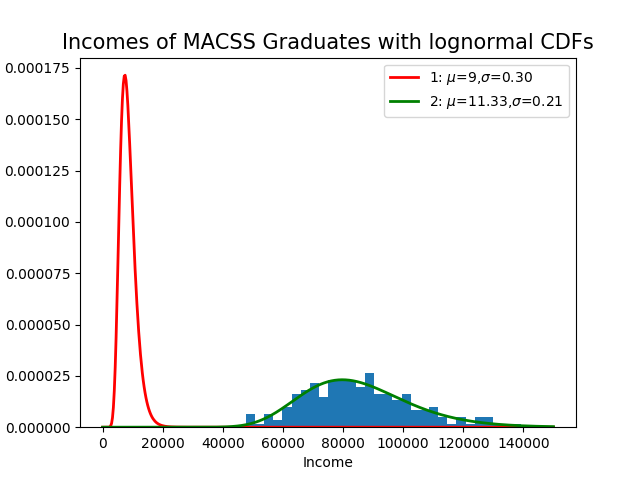
\includegraphics{images/Fig_1c.png}}}
% \end{figure}
% 18.08\% of the time I will be able to pay off the loan in 10 years.

% \noindent\textbf{Part (d).} 
% \begin{figure}[h!]\centering\captionsetup{width=4.0in}
%   \caption{\textbf{1d}}\label{FigExample}
%   \fbox{\resizebox{4.0in}{3.0in}{\includegraphics{images/Fig_1d.png}}}
% \end{figure}
% 69.87\% of the time I will be able to pay off the loan in 10 years.
 
% \begin{equation*}
%   \Omega_{j,t} = \left(\frac{\int_{m=4}^\infty(2t + 7m)dm}{\sum_{x=1}^23\sin(\theta_{j,x})}\right) + 7
% \end{equation*}
% You could refer to that object from the equation in math mode $\Omega_{j,t}$ in the sentence. Or if you wanted to talk about the equation, you could remove the asterisks, give it a label, and refer to it with references.
% \begin{equation}\label{EqCoolness}
%   \Omega_{j,t} = \left(\frac{\int_{m=4}^\infty(2t + 7m)dm}{\sum_{x=1}^23\sin(\theta_{j,x})}\right) + 7
% \end{equation}
% Look how cool equation \eqref{EqCoolness} is.

% You might want to include a table in your \LaTeX document. For this, you use the \texttt{tabular} environment.
% \begin{table}[htbp] \centering \captionsetup{width=6.0in}
% \caption{\label{TabExample}\textbf{Sweet example table}}
%   \begin{threeparttable}
%   \begin{tabular}{>{\small}l |>{\small}l >{\small}c |>{\small}r}
%     \hline\hline
%     Degrees & Time to completion & happiness (1-10) & added value (1-10) \\
%     \hline
%     High school diploma & 3.9 years & 5 & 2 \\
%     Bachelor's degree   & 3.8 years & 7 & 5 \\
%     Master's degree     & 1.7 years & 8 & 4 \\
%     PhD                 & 5.7 years & 3 & 7 \\
%     \hline\hline
%   \end{tabular}
%   \begin{tablenotes}
%     \scriptsize{\item[*]With this \texttt{threeparttable} environment, you can add nice subtext to a table.}
%   \end{tablenotes}
%   \end{threeparttable}
% \end{table}
% Lastly, you can add figures to your document. Just make sure that the reference to the figure has the right file path. Figure \ref{FigExample} is pretty nice. But, ideally, you would have something better than a pencil drawing. But you can just place any \texttt{.png} file into the \texttt{includegraphics} command.
% \begin{figure}[htb]\centering\captionsetup{width=4.0in}
%   \caption{\textbf{Great example figure}}\label{FigExample}
%   \fbox{\resizebox{4.0in}{3.0in}{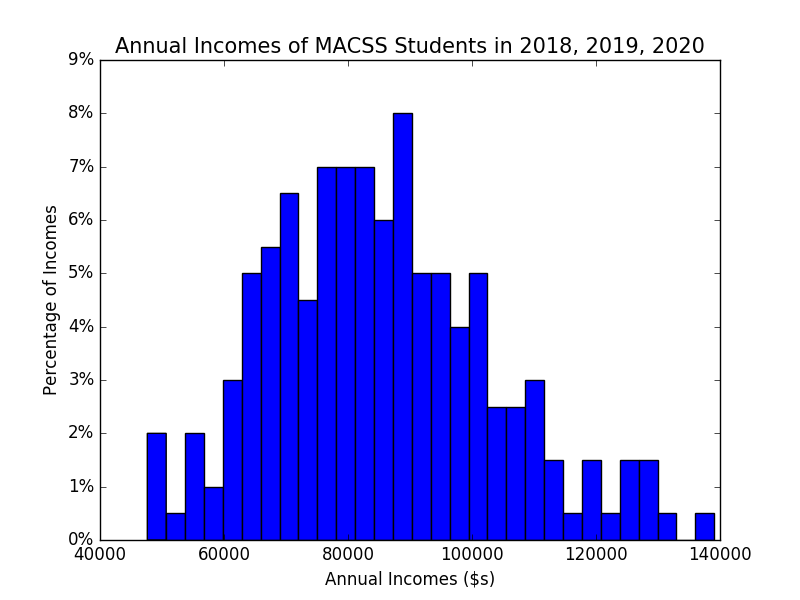
\includegraphics{images/Fig_1a.png}}}
% \end{figure}

